\begin{frame}{Muestreo de la $1^{ra}$ zona de Brillouin}
\begin{columns}[t]
    \column{0.6\textwidth}
    \begin{figure}[H]
        \centering
        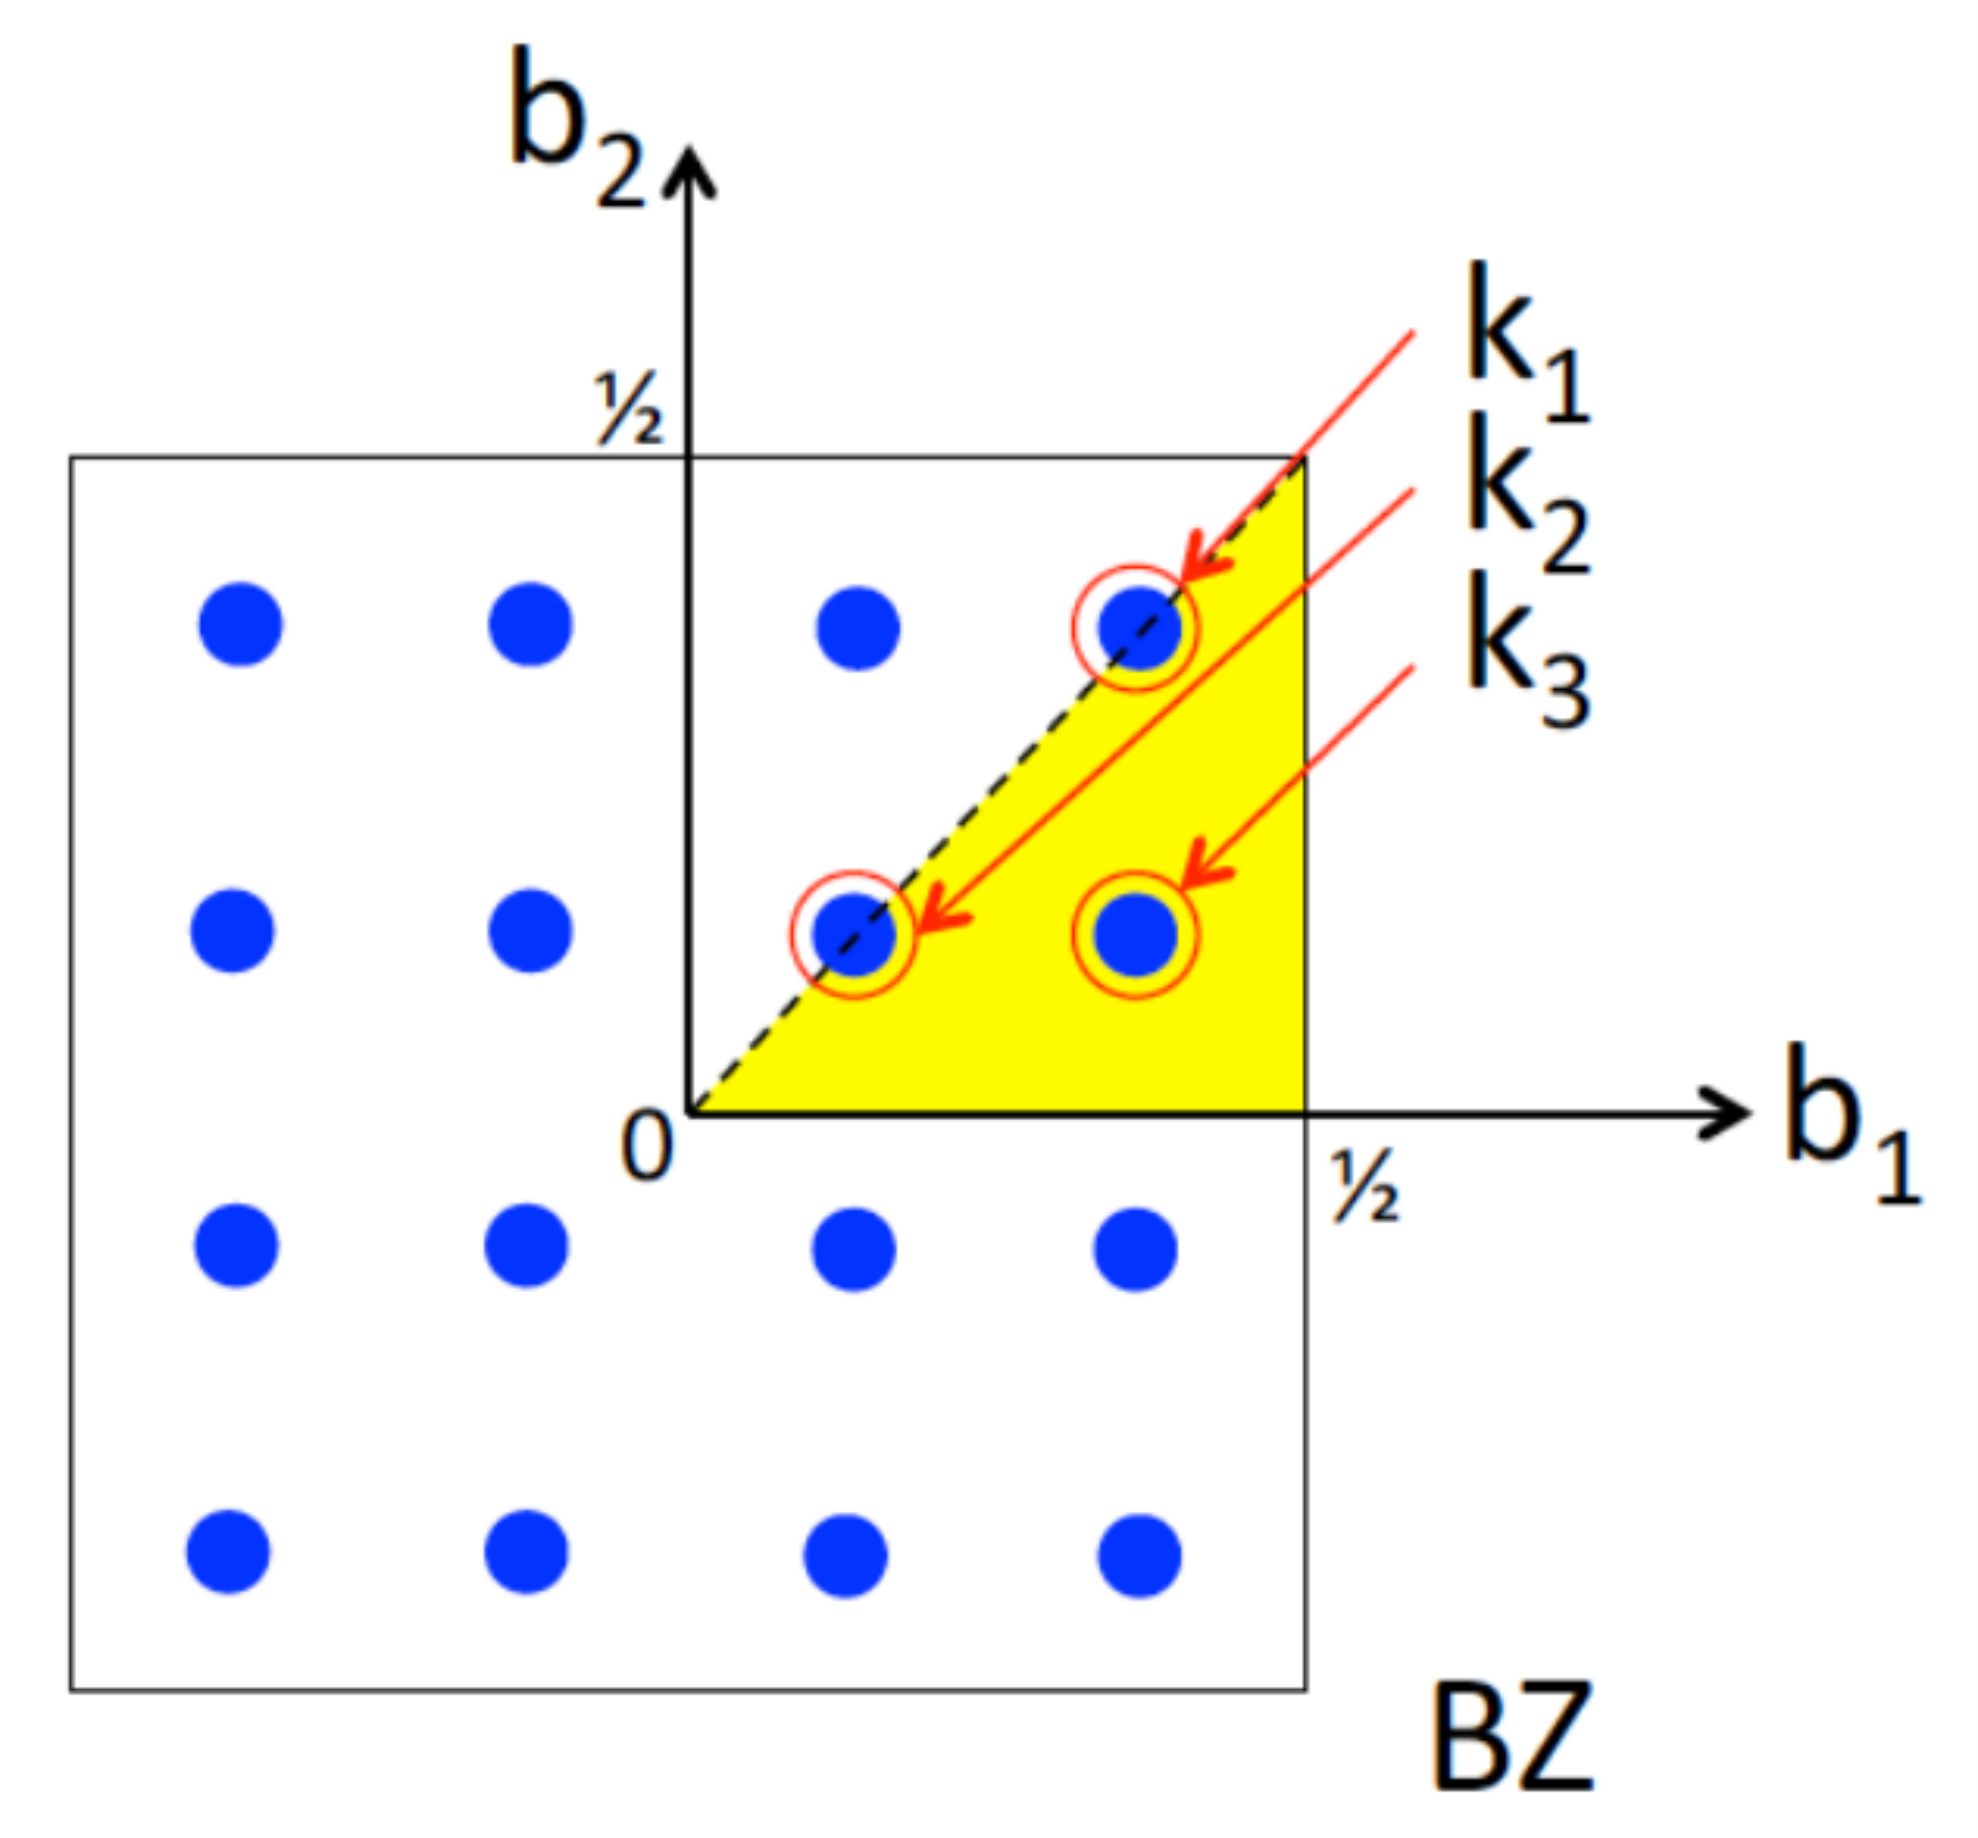
\includegraphics[width=0.9\textwidth]{contenido/teoria/img_teoria/ZonaBrillouin.png}
    \end{figure}
    \column{0.4\textwidth}
   \[ 
   \bar{A} = \int _{BZ} A(k) d(k)
   \]
   \[
   \int _{BZ} d(k) \to \sum _{K} w_{K}
   \]
   Ejemplo
   \begin{eqnarray}
   4 \times K_{1} \to w_{1} = \frac{4}{16} = \frac{1}{4} \nonumber \\
   4 \times K_{2} \to w_{2} = \frac{4}{16} = \frac{1}{4} \nonumber \\
   8 \times K_{3} \to w_{3} = \frac{8}{16} = \frac{1}{2} \nonumber
   \end{eqnarray}
\end{columns}
\[
\int _{BZ} A(k) d(k) \approx \frac{1}{4}A(K_{1}) + \frac{1}{4}A(K_{2}) + \frac{1}{2}A(K_{3})
\]
\end{frame}